\documentclass[IB,BIB]{TFUOC}%IB: CASTELLANO, CAT: CATALÁN, ENG: ANGLÈS

%Introducción de datos del trabajo
% \title{$title$} %Título del trabajo completo y tan largo como sea necesario
\title{Assessing the properties of asymptotic \break PERMANOVA test through comprehensive \break simulations in the context of genetic studies} %Título del trabajo completo y tan largo como sea necesario
\titcrt{Assessing the properties of asymptotic \break PERMANOVA through simulations} %Título corto que aparecerá a la cabecera
\author{$author$} %Nombre Estudiando Estudiante
\date{$date$}


\nomPDC{$nomPDC$} %Nombre Tutor Tutora
\nomPRA{$nomPRA$} %Nombre Profesorado Responsable
\titulac{$titulac$} %Máster en XXX
\area{$area$} %Área del trabajo
\idioma{$idioma$} %Castellano
\credits{$credits$} %15
\parcla{$parcla$} %palabra, clave, trabajo

\licenc{$licenc$}
% \licenc{ccByNcNd}
% \licenc{ccByNcSa}
% \licenc{ccByNc}
% \licenc{ccByNd}
% \licenc{ccBySa}
% \licenc{ccBy}
% \licenc{GNU}
% \licenc{copyright}
%Posibles licencias
%ccByNcNd
%ccByNcSa
%ccByNc
%ccByNd
%ccBySa
%ccBy
%GNU
%copyright


%%%%%%%%%%
% Resumen en el idioma

\abstractidioma{$abstractesp$}
% Máximo 250 palabras, con la finalidad, contexto de aplicación, metodología, resultados y conclusiones del trabajo.



% Resumen en inglés.
\abstractenglish{$abstracteng$}
% A maximum of 250 words, detailing the purpose, contexto of application, methodology, results and conclusiones of the work.

% Otras modificaciones
\renewcommand{\bibname}{Referencias}  
\renewcommand{\tablename}{Tabla}
\renewcommand{\figurename}{Figura}
\renewcommand{\listfigurename}{Índice de Figuras}
\renewcommand{\listtablename}{Índice de Tablas}

% Añadir una Lista de Ecuaciones
\usepackage{tocloft}
\newcommand{\listequationsname}{Índice de Ecuaciones}
\newlistof{myequations}{equ}{\listequationsname}
\newcommand{\myequations}[1]{
\refstepcounter{myequations}%
\par\noindent\textbf{Equation \themyequations. #1}
\addcontentsline{equ}{myequations}{\protect\numberline{\thechapter.\themyequations}#1}\par}
\setlength{\cftmyequationsnumwidth}{2.5em} % Ancho del número de ecuación en la Lista de ecuaciones

% Paquetes a cargar
\usepackage{float}
\usepackage{hyperref}
\usepackage{multicol}
\usepackage{lipsum}
\usepackage{tikz}
\usepackage{amsmath}
\usepackage{pdflscape}

% Glosario
% \usepackage[xindy]{glossaries}
\usepackage{glossaries} % Glosario y acrónimos juntos
% \usepackage[acronym]{glossaries} % Glosario y acrónimos separados
% \usepackage[toc]{glossaries}
\makeglossaries
% %%%%%%%%%%%%%%%%
% Glosario TFM %
%%%%%%%%%%%%%%%%

\makeglossaries

% Definición de términos
%%%%%%%%%%%%%%%%%%%%%%%%

% \newglossaryentry{ex}{name={sample},description={an example}}

\newglossaryentry{estadística multivariante}
  {name=estadística multivariante,
   description={La estadística multivariante o multivariada es una rama de las estadísticas que abarca la observación y el análisis simultáneos de más de una variable respuesta. La aplicación de la estadística multivariante es llamada análisis estadístico multivariante}
  }
  
\newglossaryentry{MANOVA}
  {name=MANOVA,
   description={En estadística el análisis multivariante de la varianza (Multivariate analysis of variance) es una extensión del análisis de la varianza o ANOVA para cubrir los casos donde hay más de una variable dependiente que no pueden ser combinadas de manera simple. Además de identificar si los cambios en las variables independientes tienen efectos significativos en las variables dependientes, la técnica también intenta identificar las interacciones entre las variables independientes y su grado de asociación con las dependientes}
  }

\newglossaryentry{PERMANOVA}
  {name=PERMANOVA,
   description={El análisis multivariante de la varianza con permutaciones (Permutational multivariate analysis of variance, PERMANOVA) es una prueba de permutación estadística multivariada no paramétrica. Se utiliza para comparar grupos de objetos y probar la hipótesis nula de que los centroides y la dispersión de los grupos definidos por el espacio de medida son equivalentes para todos los grupos. Un rechazo de la hipótesis nula significa que el centro y/o la dispersión de los objetos es diferente entre los grupos. De esta manera, la prueba se basa en el cálculo previo de la distancia entre cualesquier dos objetos incluidos en el experimento}
  }
  
\newglossaryentry{SNPs}
  {name=SNPs,
   description={Un polimorfismo puntual, también denominado de un solo nucleótido o SNP (Single Nucleotide Polymorphism, pronunciado snip), es una variación en la secuencia de ADN que afecta a una sola base (adenina (A), timina (T), citosina (C) o guanina (G)) de una secuencia del genoma. Sin embargo, generalmente se considera que cambios de unos pocos nucleótidos, como también pequeñas inserciones y deleciones (indels) pueden ser consideradas como SNP. Una de estas variaciones debe darse al menos en un 1 \% de la población para ser considerada como un SNP. Si no se llega al 1 \% no se considera SNP y sí una mutación puntual. En ocasiones estas variaciones de nucleótido único se asocian a otro término conocido como SNV (Single Nucleotide Variant), que a diferencia de los SNPs carece de limitaciones de frecuencia}
  }
  
\newglossaryentry{GWAS}
  {name=GWAS,
   description={En genética, un estudio de asociación del genoma completo (Genome-wide association study) o WGAS (Whole genome association study) es un análisis de una variación genética a lo largo de todo el genoma humano con el objetivo de identificar su asociación a un rasgo observable. Los GWAS suelen centrarse en asociaciones entre los polimorfismos de un solo nucleótido (SNPs) y rasgos como las principales enfermedades}
  }
  
\newglossaryentry{sQTLs}
  {name=sQTLs,
   description={Los \textit{Splicing quantitative trait loci} (sQTLs o splicing QTLs) son los loci que regulan el splicing alternativo del ARNm. Se pueden detectar utilizando datos de RNA-seq. Se han desarrollado diversos métodos para descubrir sQTLs, entre los que se incluyen: LeafCutter, Altrans, Cufflinks, y MISO}
  }
  
\newglossaryentry{RNA-seq}
  {name=RNA-seq,
   description={La secuenciación de ARN, también llamada \textit{Secuenciación del Transcriptoma Entero para Clonación al Azar}, utiliza la secuenciación masiva (NGS) para revelar la presencia y cantidad de ARN, en una muestra biológica en un momento dado. De esta manera, la RNA-seq se usa para analizar cambios en el transcriptoma, concretamente, facilita la observación de transcritos resultantes del empalme alternativo, modificación postranscripcional, fusiones génicas, mutaciones/polimorfismos de nucleótidos únicos y cambios de expresión de genes. Puede ayudar a caracterizar poblaciones diferentes de RNA como miRNA, tRNA, y rRNA, o para determinar las fronteras exón/intrón y verificar o enmendar regiones 5' y 3'}
  }

\newglossaryentry{trait}
  {name=trait,
   description={En el ámbito de la genética, un \textit{trait} o \textit{rasgo} es una característica específica de un individuo, los cuales pueden ser determinados por genes, factores ambientales o por una combinación de ambos. Se clasifican como cualitativos (e.g. el color de los ojos) o cuantitativos (e.g. la altura o la presión sanguínea). Cada uno de ellos forma parte del fenotipo general de un individuo}
  }

\newglossaryentry{pleiotropía}
  {name=pleiotropía,
   description={En biología, la pleiotropía o polifenia es el fenómeno por el cual un solo gen o alelo es responsable de efectos fenotípicos o caracteres distintos y no relacionados (e.g. la fenilcetonuria, la talasemia o anemia de células falciformes, o el albinismo de los animales que tiene un efecto pleitrópico en sus emociones haciéndolos más reactivos a su entorno)}
  }

\newglossaryentry{MANTA}
  {name=MANTA,
   description={Multivariate Asymptotic Non-parametric Test of Association. Este paquete, programado en lenguaje R, permite el cálculo no paramétrico y asimptótico del p-valor para modelos lineales multivariados}
  }
  
\newglossaryentry{MultiPhen}
  {name=MultiPhen,
   description={Paquete de R que permite testear la asociación de múltiples rasgos. Realiza pruebas de asociación genética entre SNPs y múltiples fenotipos (por separado o en conjunto)}
  }

\newglossaryentry{mvLMMs}
  {name=mvLMMs,
   description={Los modelos lineales mixtos multivariados son poderosas herramientas para probar asociaciones entre polimorfismos de núcleo único y múltiples fenotipos correlacionados mientras controlan la estratificación de la población en estudios de asociación de todo el genoma}
  }

\newglossaryentry{MTAR}
  {name=MTAR,
   description={Marco desarrollado para el análisis multi-trait de RVAS. Se basa en un meta-modelo analítico de efectos aleatorios que utiliza diferentes estructuras de correlación de los efectos genéticos para representar un amplio espectro de patrones de asociación a través de rasgos y variantes}
  }

\newglossaryentry{MOSTest}
  {name=MOSTest,
   description={Es una herramienta para unir el análisis genético de múltiples rasgos, que utiliza el análisis multivariado para aumentar la potencia, y así poder descubrir los loci asociados}
  }

\newglossaryentry{error de tipo I}
  {name=error de tipo I,
   description={En un estudio de investigación, el error de tipo I, también denominado error de tipo alfa (\alpha) o falso positivo, es el error que se comete cuando el investigador rechaza la hipótesis nula (*H*$_{0}$: el supuesto inicial) siendo esta verdadera en la población. Es equivalente a encontrar un resultado falso positivo, porque el investigador llega a la conclusión de que existe una diferencia entre las hipótesis cuando en realidad no existe. Se relaciona con el nivel de significancia estadística}
  }

\newglossaryentry{error de tipo II}
  {name=error de tipo II,
   description={En un estudio de investigación, el error de tipo II, también llamado error de tipo beta (donde \beta es la probabilidad de que exista este error) o falso negativo, se comete cuando el investigador no rechaza la hipótesis nula (*H*$_{0}$: el supuesto inicial) siendo esta falsa en la población. Es equivalente a la probabilidad de un resultado falso negativo, ya que el investigador llega a la conclusión de que ha sido incapaz de encontrar una diferencia que existe en la realidad. De forma general y dependiendo de cada caso, se suele aceptar en un estudio que el valor del error beta esté entre el 5 y el 20 \%}
  }

\newglossaryentry{potencia}
  {name=potencia,
   description={La potencia o poder de una prueba estadística es la probabilidad de que la hipótesis alternativa sea aceptada cuando la hipótesis alternativa es verdadera, es decir, la probabilidad de no cometer un error del tipo II. En general, es una función de las distribuciones posibles, a menudo determinada por un parámetro, bajo la hipótesis alternativa. A medida que aumenta la potencia, las posibilidades de que se presente un error del tipo II se reducen (disminución de la tasa de falsos negativos \beta), de esta manera, la potencia se representa como $1-\beta$ (sensibilidad). El análisis de la potencia se puede utilizar para calcular el tamaño mínimo de la muestra necesario para que uno pueda detectar razonablemente un efecto de un determinado tamaño, o también para calcular el tamaño del efecto mínimo que es probable que se detecte en un estudio usando un tamaño de muestra dado. Además, el concepto de \textit{alimentación} se utiliza para hacer comparaciones entre diferentes procedimientos de análisis estadísticos (e.g. entre una prueba paramétrica y una no paramétrica de la misma hipótesis}
  }

\newglossaryentry{pseudo-F}
  {name=pseudo-F,
   description={En el análisis multivariante de la varianza con permutacionesa (\textit{PERMANOVA}), el estadístico de prueba es una pseudo-ratio F, similar a la relación F en ANOVA. Compara la suma total de diferencias cuadradas (o diferencias de orden) entre objetos pertenecientes a diferentes grupos con la de objetos que pertenecen al mismo grupo. Las F-ratios más grandes indican una separación de grupo más pronunciada, sin embargo, la significación estadística de esta relación suele ser más interesante que su magnitud}
  }

\newglossaryentry{valores p}
  {name=valores p,
   description={En estadística general y contrastes de hipótesis, los valores p (p, p-valor, valor de p consignado, o p-value) se define como la probabilidad de que un valor estadístico calculado sea posible dada una hipótesis nula cierta. Ayuda a diferenciar resultados que son producto del azar del muestreo, de resultados que son estadísticamente significativos. Alternativamente, se define como la probabilidad de observar los resultados del estudio, u otros más alejados de la hipótesis nula, si la hipótesis nula fuera cierta, de manera que si este cumple con la condición de ser menor que un nivel de significancia impuesto arbitrariamente, este se considera como un resultado estadísticamente significativo y, por lo tanto, permite rechazar la hipótesis nula}
  }


% ==> SEGUIR CON GLOSARIO A PARTIR DEL ESTADO DEL ARTE
  
  
% ------------------------------------------------------------------------------------------------------------------------------------------------

% Cómo especificar los términos del glosario en el documento LATEX:

% \gls{ }
% To print the term, lowercase. For example, \gls{maths} prints mathematics when used.

% \Gls{ }
% The same as \gls but the first letter will be printed in uppercase. Example: \Gls{maths} prints Mathematics

% \glspl{ }
% The same as \gls but the term is put in its plural form. For instance, \glspl{formula} will write formulas in your final document.

% \Glspl{ }
% The same as \Gls but the term is put in its plural form. For example, \Glspl{formula} renders as Formulas.


% Estilos del glosario:

% The command \glossarystyle{style} must be inserted before \printglossaries. Below a list of available styles:

% list. Writes the defined term in boldface font
% altlist. Inserts newline after the term and indents the description.
% listgroup. Group the terms based on the first letter.
% listhypergroup. Adds hyperlinks at the top of the index.


% Imprimir el glosario en el documento:
% 
% \printglossary


% Cómo especificar los acrónimos en el documento LATEX:

% \acrlong{ }
% Displays the phrase which the acronyms stands for. Put the label of the acronym inside the braces. In the example, \acrlong{gcd} prints Greatest Common Divisor.

% \acrshort{ }
% Prints the acronym whose label is passed as parameter. For instance, \acrshort{gcd} renders as GCD.

% \acrfull{ }
% Prints both, the acronym and its definition. In the example the output of \acrfull{lcm} is Least Common Multiple (LCM).

% To print the list of acronyms use the command
% 
% \printglossary[type=\acronymtype]


% Cambiar el nombre del glosario y del título en TOC:

% \printglossary[title=Special Terms, toctitle=List of terms]

% Notice that the command \printglossary has two comma-separated parameters:
% title=Special Terms is the title to be displayed on top of the glossary.
% toctitle=List of terms this is the entry to be displayed in the table of contents. 
 % 1a opción para cargar el glosario externo
\loadglsentries{TFM_ glossary} % 2a opción para cargar el glosario externo

\floatplacement{figure}{H}
\DeclareUnicodeCharacter{0301}{*************************************}
%\setcounter{MaxMatrixCols}{20} % Cambia la dimensión máxima de una matriz (columnas), por defecto 10.
%\usepackage[spanish]{babel}
  
% Bibliografía
% \usepackage{biblatex}
% \usepackage{biblatex}
% \addbibresource{TFM.bib}
% \addbibresource{$bibliography$}


\begin{document}

\estructura\label{fitxa}


\newpage

\tableofcontents


% %%%%%%%%
% % PEC1 %
% %%%%%%%%

% \chapter{PEC 1}
% 
% Objetivos principales de la primera PEC:
% 
% {\footnotesize
% \begin{itemize}
%     \item Definir claramente cuál es la temática del trabajo, justificar su interés y/o relevancia y qué se quiere conseguir al finalizar el TFM.     \item Definir los objetivos del trabajo de forma concisa.
%     \item Definir y planificar las tareas que proponéis para conseguir estos objetivos.
%     \item Definir y valorar los riesgos y determinar las acciones de mitigación.
% \end{itemize}}
% 
% 
% \section{Tabla informativa del trabajo}
% 
% Se proporciona una tabla con la siguiente información:
% 
% {\footnotesize
% \begin{itemize}
%     \item Título que refleja el contenido y finalidad del presente TFM.
%     \item Selección \textit{a priori} de las palabras clave en inglés (\textit{\textbf{keywords}}) que intentan resumir de forma genérica los conceptos más relevantes del trabajo. Este conjunto es susceptible de ser modificado a medida que avance el proyecto.
%     \item Otra información relevante: {\textit{Nombre del autor/a, Nombre del tutor/a de TF, Nombre del/de la PRA, Fecha de entrega, Titulación o programa, Área del trabajo final e Idioma del trabajo}}
% \end{itemize}}
% 
% Dicha tabla puede encontrarse en la \hyperref[fitxa]{sección pertinente}.


% \section{Contexto y Justificación del Trabajo}
% % Contextualizad el TFM, explicad a qué ámbito pertenece, y justificad su interés: explicad por qué el trabajo que habéis elegido es interesante.
% 
% 
% % Propuesta de TFM (D. Garrido y M. Calvo):
% %
% %  Título: Assessing the properties of asymptotic PERMANOVA test through comprehensive
% %          simulations in the context of genetic studies
% %
% %  Objetivos principales:
% %
% %    - Estudio de potencia con distintas transformaciones (sqrt, log, datos composicionales, etc.)
% %    - Estudio de la pérdida de potencia con respecto a MANOVA con P-valores pequeños
% %    - Evaluación comparativa del método de Davies y el propuesto en Yang J. et al.
% %      (implementación en C/C++)
% %
% %  Comentarios PEC1 (D. Garrido y M. Calvo):
% %
% %    - Acordarse que en todo caso trabajamos con la versión asintótica de PERMANOVA,
% %                no con PERMANOVA!!! 
% %
% %    - Descripción más detallada:
% %
% %      a) GWAS y QTL mapping
% %      b) Cómo en estos análisis se usan sobre todo métodos univariantes
% %      c) Ventajas de las aproximaciones multivariantes
% %      d) Limitaciones (parametricas, running time)
% %      e) Cómo PERMANOVA puede ser una buena alternativa, pero necesita permutaciones,
% %         razón por la que hemos desarrollado MANTA (= asymptotic PERMANOVA)
% %      f) Aquí entra tu TFM: estudiar las propiedades de MANTA en algunos escenarios,
% %         comparar transformaciones, estudiar pérdida de potencia vs MANOVA y otros métodos
% %         (reportada en este artículo: https://www.nature.com/articles/s41588-022-01154-4), 
% %         implementaciones (e.g. Farebrother -current- vs Saddlepoint), etc.
% %         Nosotros ya hicimos benchmark Davies vs Farebrother vs Imhof vs Liu, aunque se puede ampliar,
% %         el objetivo fundamental es comparar Farebrother con Saddlepoint.
% 
% 
% El tema escogido para la realización del TFM se enmarca en el área del ánalisis de datos ómicos y, en particular, en el análisis estadístico multivariante, principalmente \textbf{MANOVA} y la versión asintótica de \textbf{PERMANOVA}, aplicado al estudio de asociaciones entre los polimorfismos de un solo nucleótido (\textbf{SNPs}) del genoma completo (\textbf{GWAS}, \textit{Genome-wide association study}) y algunos rasgos característicos, como son las principales enfermedades humanas, así como en la detección de \textit{Splicing quantitative trait loci} (\textbf{sQTLs} o \textbf{splicing QTLs}) utilizando datos \textbf{RNA-seq}.
% 
% \newpage
% 
% %      a) GWAS y QTL mapping
% %      b) Cómo en estos análisis se usan sobre todo métodos univariantes
% 
% Habitualmente, tanto las investigaciones basadas en (\textbf{GWAS}) como en \textbf{sQTLs}, se han realizado con la finalidad de comprobar la asociación entre los polimorfismos de un solo nucleótido (\textbf{SNPs}) con diferentes variantes genéticas mediante el estudio de un único rasgo (única variable o \textit{trait}), con lo que los análisis estadísticos correspondientes llevados a cabo suelen utilizar, lógicamente, los principales métodos univariantes disponibles (sumario estadístico basado en tablas de distribución de frecuencias, estadísticos de centralización o dispersión, etc.).
% 
% De este modo, este tipo de estudios al centrarse en un solo \textit{trait} de todos los disponibles en el gran volumen de datos sobre fenotipos utilizable, no permiten tratar la posible relación causa-efecto subyacente, obteniendo un análisis méramente descriptivo. \\
% 
% %      c) Ventajas de las aproximaciones multivariantes
% %      d) Limitaciones (parametricas, running time)
% %      e) Cómo PERMANOVA puede ser una buena alternativa, pero necesita permutaciones,
% %         razón por la que hemos desarrollado MANTA (= asymptotic PERMANOVA)
% 
% Alternativamente, gracias a la gran cantidad de datos disponibles últimamente con perfiles genómicos complejos (alta diversidad de rasgos moleculares), la necesidad de encontrar correlaciones entre las diferentes variables analizables y los rasgos de interés, ha resultado en un crecimiento en la utilización de métodos multivariantes para su análisis estadístico.
% 
% Las principales ventajas con respecto al enfoque univariante clásico, para poder determinar la posible estructura de correlaciones subyacente en los datos, pueden enumerarse como sigue:
% 
% {\small
% \begin{itemize}
%     \item Mayor potencia estadística para detectar asociaciones genéticas.
%     \item Ofrece ventajas en el estudio de la \textit{pleiotropía} (cuando el gen o alelo considerado es responsable de efectos fenotípicos o caracteres distintos y, a priori, no relacionados).
%     \item Resulta de utilidad incluso cuando solo un pequeño grupo de los rasgos se ve afectado por el genotipo de interés.
%     \item Permite el análisis a través de múltiples capas fenotípicas en bloque, dando luz sobre los mecanismos moleculares activados por las variantes genéticas consideradas.
%     \item Posibilita la caracterización de los efectos genéticos sobre un mismo rasgo cuando este es medido en diferentes condiciones ambientales o entornos.
%     \item Requiere de menos pruebas individuales, lo que disminuye las de carácter múltiple.
% \end{itemize}}
% 
% Contrariamente, del uso de los métodos más habitualmente utilizados para estudiar estas asociaciones genéticas multirasgo emergen diversos inconvenientes, entre los cuales destacan:
% 
% {\small
% \begin{itemize}
%     \item Los métodos que modelan el genotipo como variable dependiente comprobando a su vez la asociación con una suma ponderada de fenotipos (\textbf{MV-PLINK} o análisis de correlación canónica, y \textbf{MultiPhen} que utiliza la regresión ordinal) adolecen de la posibilidad de evaluar diseños complejos que presentan mutiples interacciones entre el genotipo y otras covariables. 
%     \item Tanto el análisis multivariante de la varianza (\textbf{MANOVA}), como el de los modelos multivariantes lineales mixtos (\textbf{LMM}), resultan ser más tolerantes a estos diseños complejos al tratar los fenotipos como variables dependientes, introduciendo de froma natural el posible parentesco genético entre los individuos analizados. Esta ventaja se torna inconveniente para grandes conjuntos de datos, sobre todo para el método \textbf{LMM}, cuya continua mejora en su implementación computacional sigue requiriendo de tiempos excesivamente altos. 
%     \item La pluralidad de los métodos de regresión multivariante presuponen una normalidad en la distribución de los errores del modelo que puede no llegar a cumplirse. Todo y que pueden aplicarse transformaciones individuales a cada rasgo estudiado, no puede garantizarse la normalidad multivariante, lo que resulta en una reducción de la potencia estadística en comparación con el modelo aplicado a los rasgos no transformados.
%     \item Hasta el momento, las diversas implementaciones de \textbf{métodos bayesianos} para el estudio de asociaciones multirasgo no han sido satisfactorias, requiriendo siempre un tiempo elevado de cálculo debido al coste computacional que implican.
%     \item Para los métodos \textit{Various Multi-Trait Association tests in R} (\textbf{MTAR}) o \textit{Multivariate Omnibus Statistical Test} (\textbf{MOSTest}) existe la necesidad de garantizar la normalidad multivariante asintótica cuando se utilizan los sumarios estadísticos univariantes, lo que no es trivial, sumado a que evitar la aparición de sesgos en la estimación de correlaciones de rasgos a partir de esta clase de estadísticos no es sencillo (afectaciones de heredabilidad de los rasgos, patrones de desequilibrio de ligamiento, etc.).
% \end{itemize}}
% 
% Con todo lo anterior, resulta evidente la necesidad de disponer de un método no paramétrico adecuado tanto para los estudios basados en (\textbf{GWAS}) como en \textbf{sQTLs}. El modelo de \textit{análisis multivariante permutacional de la varianza} o \textbf{PERMANOVA} (\cite{anderson_new_2001}) amplía el modelo lineal factorial univariante a múltiples dimensiones sin requerir una distribución de probabilidad conocida de las variables dependientes, introduciendo un enfoque basado en la distancia, poniendo a prueba la hipótesis de ausencia de efectos mediante un procedimiento de permutación basado en un estadístico \textbf{pseudo-F}, en el que las sumas de cuadrados del \textbf{ANOVA} se sustituyen por sumas de interdistancias entre observaciones.\\
% Pese a ser exitoso en muchos estudios, dando buenos resultados en un tiempo de cálculo reducido para diseños fijos unidireccionales, resulta inviable en los estudios actuales, donde el mayor tamaño y complejidad de los conjuntos de datos requiere una precisión para el cálculo del valor p que este procedimiento permutacional no puede alcanzar en las condiciones requeridas.
% 
% El punto de partida del presente trabajo radica en los diversos estudios realizados con el fin de superar esta limitación. En concreto: sendos artículos de Garrido-Martín, D. \textit{et al.} (\cite{garrido-martin_fast_2022} y \cite{garrido-martin_identification_2021}), y el trabajo de Monlong, J. \textit{et al.} \cite{monlong_identification_2014}. Donde, gracias al programa \textit{Multivariate Asymptotic Non-parametric Test of Association} o \textbf{MANTA} (\cite{garrido-martin_manta_2023}, desarrollado principalmente en R), se estudia mediante diversas simulaciones (\cite{garrido-martin_manta-sim_2022}) de diseños complejos la distribución asintótica de la estadística de pruebas PERMANOVA en el caso de la distancia euclídea (valores P de carácter no paramétrico y asintótico para modelos lineales multivariados), obteniendo resultados igualmente válidos tras cualquier transformación de los datos que preserve la independencia de las observaciones.
% 
% %      f) Aquí entra tu TFM: estudiar las propiedades de MANTA en algunos escenarios,
% %         comparar transformaciones, estudiar pérdida de potencia vs MANOVA y otros métodos
% %         (reportada en este artículo: https://www.nature.com/articles/s41588-022-01154-4), 
% %         implementaciones (e.g. Farebrother -current- vs Saddlepoint), etc.
% %         Nosotros ya hicimos benchmark Davies vs Farebrother vs Imhof vs Liu, aunque se puede ampliar,
% %         el objetivo fundamental es comparar Farebrother con Saddlepoint.
% 
% La finalidad principal será ahondar en estos estudios, yendo más allá en al menos los siguientes aspectos:
% 
% {\small
% \begin{itemize}
%     \item Estudiar las propiedades de MANTA en algunos escenarios, determinando cómo los diferentes tipos de transformaciones de datos afectan a los resultados obtenidos, y dilucidar si existe algún protocolo privilegiado en las simulaciones implementadas.
%     \item Estudiar la pérdida de potencia de la versión asintótica de PERMANOVA con respecto a MANOVA y otros métodos, profundizando en la afectación de la variación del nivel de significación considerado sobre la potencia de cada uno.
%     \item Comparar los resultados obtenidos con respecto al cálculo de la distribución de las formas cuadráticas entre el método Farebrother (implementado para la versión asintótica de PERMANOVA con MANTA) y el de Saddlepoint.
%     \item Extender el punto anterior, ampliando la comparativa Farebrother vs Saddlepoint a otros métodos: métodos exactos como el de Davies, R. B. (\cite{davies_numerical_1973}, \cite{davies_algorithm_1980}), o aproximaciones numéricas como la de Liu–Tang–Zhang (\cite{qi_genetic_2022}), el método de Imhof, etc.
%     \item Partiendo del caso de estudio anterior, y secundariamente, se llevaría a cabo la implementación del método más óptimo en el paquete MANTA ya existenete, en caso de que este exista.
% \end{itemize}}


% \section{Descripción general}
% % Explicad a grandes rasgos en qué consistirá el TFM. Este punto no debe confundirse con una introducción, sino que también debe explicar brevemente como planeáis que sea el trabajo.
% 
% 
% %  Comentarios PEC1 (D. Garrido y M. Calvo):
% %
% %    - En este contexto yo no añadiría los objetivos como tal, describe un poco si quieres pero
% %      ponlos en el apartado correspondiente
% %    - Quizás puedes definir un objetivo general, que sea estudiar las propiedades de MANTA en
% %      distintos contextos de simulación [...] y mejorar la implementación actual y luego añadir
% %      los objetivos (que ahora llamas principales) como específicos. O alternativamente desarrollar
% %      un par de objetivos específicos por cada uno de los principales.
% 
% 
% Siguiendo las pautas del punto anterior, este TFM consistirá en un trabajo principalmente teórico, en el cual se profundizará en aspectos concretos de los estudios ya referenciados (\cite{garrido-martin_fast_2022}, \cite{garrido-martin_identification_2021}), \cite{monlong_identification_2014}), con el objetivo de determinar la validez de la versión asintótica del método PERMANOVA (implementado en el paquete MANTA) con respecto a otros métodos similares bajo un mismo conjunto de simulaciones complejas basadas en datos de escenarios reales.
% 
% 
% \section{Objetivos}
% % Explicad claramente tanto los objetivos generales como los específicos:
% % Objetivos generales: Deben ser pocos (quizás un par o máximo tres) y suficientemente amplios para cubrir todo el alcance del proyecto. Deben estar redactados de forma concreta y evaluable.
% % Objetivos específicos: desglosad cada objetivo general en otros más concretos (no confundir con tareas). Se deben redactar con un verbo en infinitivo de significado medible (no puede ser por ejemplo “saber” porque no se puede medir  o evidenciar su cumplimiento).
% 
% Se han considerado, al menos, tres objetivos principales:
% 
% {\small
% \begin{itemize}
%     \item Estudiar las propiedades de MANTA en algunos escenarios, determinando cómo los diferentes tipos de transformaciones de datos afectan a los resultados obtenidos, y dilucidar si existe algún protocolo privilegiado en las simulaciones implementadas.
%     \item Estudiar la pérdida de potencia de la versión asintótica de PERMANOVA con respecto a MANOVA y otros métodos, profundizando en la afectación de la variación del nivel de significación considerado sobre la potencia de cada uno.
%     \item Comparar los resultados obtenidos con respecto al cálculo de la distribución de las formas cuadráticas entre el método Farebrother (implementado para la versión asintótica de PERMANOVA con MANTA) y el de Saddlepoint.
% \end{itemize}}
% 
% Y los siguientes objetivos secundarios:
% 
% {\small
% \begin{itemize}
%     \item Extender el punto anterior, ampliando la comparativa Farebrother vs Saddlepoint a otros métodos: métodos exactos como el de Davies, R. B. (\cite{davies_numerical_1973}, \cite{davies_algorithm_1980}), o aproximaciones numéricas como la de Liu–Tang–Zhang (\cite{qi_genetic_2022}), el método de Imhof, etc.
%     \item Partiendo del caso de estudio anterior, y secundariamente, se llevaría a cabo la implementación del método más óptimo en el paquete MANTA ya existenete, en caso de que este exista.
% \end{itemize}}


% \section{Enfoque y método a seguir}
% % Indicad cuáles son las posibles estrategias para llevar a cabo el trabajo e indicar cuál es la elegida. Valorad por qué ésta es la más apropiada para lograr los objetivos.
% 
% 
% %  Comentarios PEC1 (D. Garrido y M. Calvo):
% %
% %    - Desarrolla una lista de tareas y método a seguir, así como una planificación orientativa (Gannt).
% %      Entiendo que serán preliminares, pero en cualquier caso estaría bien que te plantearas las
% %      distintas tareas, así como que hicieras una pequeña evaluación de riesgos.
% 
% Se ha enfocado el trabajo siguiendo las pautas que las diferentes entregas programadas (\textit{Pruevas de Evaluación Continua} o \textbf{PEC}) por la UOC marcan, de manera que se han establecido los siguientes bloques de trabajo:
% 
% % Primera entrega: PEC1 - Definición y plan de trabajo
% % Primera tutoría: propuesta oficial de TFM (título, objetivos principales, etc.).
% % Redacción de la PEC1.
% % Entrega de la PEC1.
% % Enmiendas sobre la entrega de la PEC1.
% % Corrección de la PEC1 según las sugerencias realizadas por los tutores.
% % Entrega corregida.
% % 
% % Segunda entrega: PEC2 - Desarrollo del trabajo - Fase 1
% % Redacción de la memoria: adaptación del contenido de la PEC1 a los correspondientes apartados, y redacción del capítulo "Estado del arte".
% % Inicio de las pruebas en R con MANTA, primer objetivo: estudiar las propiedades de MANTA en algunos escenarios comparando diferentes transformaciones de los datos.
% % Redacción de la memoria: inclusión, si cabe, de los primeros resultados obtenidos.
% % Entrega de la PEC2.
% % 
% % Tercera entrega: PEC3 - Desarrollo del trabajo - Fase 2
% % Pruebas en R con MANTA, segundo objetivo: estudiar la pérdida de potencia de la versión asintótica de PERMANOVA con respecto a MANOVA y otros métodos.
% % Valorar, tras los resultados obtenidos para el segundo objetivo, la posibilidad de implementar mejoras en MANTA.
% % Pruebas en R con MANTA, tercer objetivo: comparar los resultados obtenidos con respecto al cálculo de la distribución de las formas cuadráticas entre el método Farebrother (implementado para la versión asintótica de PERMANOVA con MANTA) y el de Saddlepoint.
% % Pruebas en R con MANTA, otros objetivos: extender el tercer objetivo, ampliando la comparativa Farebrother vs Saddlepoint a otros métodos (Davies, Imhof, Liu, etc.).
% % Redacción de la memoria: adaptación del contenido de la PEC1 y PEC2 a los correspondientes apartados, redacción del capítulo "Resultados" e inicio del apartado "Discusión".
% % Entrega de la PEC3.
% % 
% % Cuarta entrega: PEC4 - Cierre de la memoria y de la presentación
% % Redacción de la memoria: adaptación del contenido de la PEC1, PEC2 y PEC3 a los correspondientes apartados, completando la redacción de los capítulos  "Discusión", "Conclusiones y trabajos futuros" y "Glosario".
% % Creación de la presentación según la memoria final y los criterios establecidos.
% % Entrega de la memoria y la presentación (sendas copias en el REC y la aplicación Present@).
% 
% {\small
% \begin{itemize}
%     \item Primera entrega: PEC1 - Definición y plan de trabajo (10 \% de dedicación).
%     \item Segunda entrega: PEC2 - Desarrollo del trabajo - Fase 1 (35 \% de dedicación).
%     \item Tercera entrega: PEC3 - Desarrollo del trabajo - Fase 2 (35 \% de dedicación).
%     \item Cuarta entrega: PEC4 - Cierre de la memoria y de la presentación (15 \% de dedicación).
%     \item Defensa pública (5 \% de dedicación).
% \end{itemize}}
% 
% Se puede encontrar una planificación más detallada en la siguiente sección.
% 
% 
% \newpage
% \begin{landscape}
% 
% \section{Planificación}\label{Planificación}
% % Desglosad las tareas que vais a hacer para conseguir vuestros objetivos y proponed una planificación temporal. 
% % Tareas: Enumerad las diversas tareas en que se han desglosado los objetivos y la duración que se asigna a cada una. Tiene que haber una coherencia numérica entre objetivos generales, objetivos específicos y tareas.
% % Calendario: Es recomendable usar un programa específico de planificación para generar un diagrama de Gantt que se pueda insertar en el documento.
% % Hitos: Los hitos marcan los estados intermedios del proyecto y permiten avanzar en sucesivas etapas de resultados prácticos, por ejemplo, tomando decisiones relevantes. Es imprescindible que seáis estrictos en el cumplimiento de las fechas que os marquéis. Será importante que os baséis en el Plan Docente y concretamente en las fechas clave que se indican allá para elaborar vuestra planificación.
% % Análisis de riesgos: Enumerad y comentad qué factores pueden repercutir negativamente en el seguimiento del plan de trabajo y en la consecución del proyecto. Hay dos factores que tienen influencia en cualquier proyecto: el alcance del proyecto  y el tiempo del que disponéis para realizarlo. Hay otros riesgos asociados a las características específicas de cada TFM y al método de investigación y/o de desarrollo que se utiliza. Igual que los objetivos, deben ser concretos. 
% 
% Una planificación orientativa de las tareas que conforman cada bloque de trabajo específico, en parte basada en la estructura de las diferentes PEC a entregar, puede encontrarse en \ref{fig:GANTT_TFM}. \footnote{Esta página se muestra de forma apaisada deliberadamente, con tal de acomodar la imagen correctamente.}
% 
% \begin{figure}[!htbp]
%     \centering
%     \includegraphics[width=22truecm]{GANTT_TFM.png}
%     \caption{Planificación orientativa de las tareas a realizar para la consecución de la memoria y presentación del presente TFM.}
%     \label{fig:GANTT_TFM}
% \end{figure}
% 
% 
% \newpage
% \end{landscape}

% \section{Resultados esperados}
% % En este apartado debéis concretar qué se obtendrá al final del proyecto. Tienen que ser ítems tangibles y medibles de lo que se espera obtener. Recordad que estos resultados deberán incluir los entregables que os pedimos al final del trabajo:
% % Plan de trabajo.
% % Memoria.
% % Producto, si es que hay un producto resultado que no se incluye en la memoria, por ejemplo un artículo, un software desarrollado, etc.
% % Presentación virtual.
% 
% Productos que se esperan obtener al final del proyecto:
% 
% {\small
% \begin{itemize}
%     \item Plan de trabajo: distribución de tareas según los objetivos determinados, puntos clave y tiempos necesarios. Disponible en la sección \hyperref[Planificación]{Planificación}.
%     \item Memoria: producto derivado de todas las entregas parciales (PEC), basado en la estructura recomendada por la UOC.
%     \item Producto: aún sin ser un objetivo principal, puede llegar a obtenerse una iteración mejorada del programario utilizado ya existente.
%     \item Presentación virtual del TFM: basada en la memoria producida y según los criterios establecidos por la UOC.
% \end{itemize}}


% \section{Bibliografía}
% 
% Selección preliminar basada en la bibliografía de partida recomendada por los tutores (\cite{garrido-martin_fast_2022}, \cite{garrido-martin_identification_2021}, \cite{monlong_identification_2014}, \cite{anderson_new_2001}, \cite{anderson_generalized_2003}, \cite{hoffmann_archaea_2013}, \cite{casale_multivariate_2016}, \cite{stephens_unified_2013}, \cite{hackinger_statistical_2017}, \cite{garrido_martin_multivariate_2020}), otros artículos estrechamente relacionados con alguno de los objetivos marcados (\cite{duchesne_computing_2010}, \cite{kuonen_saddlepoint_1999}, \cite{qi_genetic_2022}, \cite{hothorn_simultaneous_2008}), y una selección inicial de referencias sobre estadística, análisis multivariante y genética (\cite{freund_statistical_2022}, \cite{herzog_understanding_2019}, \cite{mills_introduction_2020}, \cite{sullivan_fundamentals_2022}, \cite{aldas_manzano_alisis_2017}, \cite{cuadras_nuevos_2007}, \cite{noauthor_encyclopedia_2019}).


%%%%%%%
% TFM %
%%%%%%%

%%%%%%%%%%%%%%%%%%%%%%%%%%%%%%%%%%%%%%%%%%
% Primera parte: Introducción  <--> PEC1 %
%%%%%%%%%%%%%%%%%%%%%%%%%%%%%%%%%%%%%%%%%%


\chapter{Introducción}


\section{Contexto y justificación del trabajo}

% Contextualizad el TFM, explicad a qué ámbito pertenece, y justificad su interés: explicad por qué el trabajo que habéis elegido es interesante.


% Propuesta de TFM (D. Garrido y M. Calvo):
%
%  Título: Assessing the properties of asymptotic PERMANOVA test through comprehensive
%          simulations in the context of genetic studies
%
%  Objetivos principales:
%
%    - Estudio de potencia con distintas transformaciones (sqrt, log, datos composicionales, etc.)
%    - Estudio de la pérdida de potencia con respecto a MANOVA con P-valores pequeños
%    - Evaluación comparativa del método de Davies y el propuesto en Yang J. et al.
%      (implementación en C/C++)
%
%  Comentarios PEC1 (D. Garrido y M. Calvo):
%
%    - Acordarse que en todo caso trabajamos con la versión asintótica de PERMANOVA,
%                no con PERMANOVA!!! 
%
%    - Descripción más detallada:
%
%      a) GWAS y QTL mapping
%      b) Cómo en estos análisis se usan sobre todo métodos univariantes
%      c) Ventajas de las aproximaciones multivariantes
%      d) Limitaciones (parametricas, running time)
%      e) Cómo PERMANOVA puede ser una buena alternativa, pero necesita permutaciones,
%         razón por la que hemos desarrollado MANTA (= asymptotic PERMANOVA)
%      f) Aquí entra tu TFM: estudiar las propiedades de MANTA en algunos escenarios,
%         comparar transformaciones, estudiar pérdida de potencia vs MANOVA y otros métodos
%         (reportada en este artículo: https://www.nature.com/articles/s41588-022-01154-4), 
%         implementaciones (e.g. Farebrother -current- vs Saddlepoint), etc.
%         Nosotros ya hicimos benchmark Davies vs Farebrother vs Imhof vs Liu, aunque se puede ampliar,
%         el objetivo fundamental es comparar Farebrother con Saddlepoint.


El tema escogido para la realización del TFM se enmarca en el área del ánalisis de datos ómicos y, en particular, en el análisis estadístico multivariante, principalmente \textbf{MANOVA} y la versión asintótica de \textbf{PERMANOVA}, aplicado al estudio de asociaciones entre los polimorfismos de un solo nucleótido (\textbf{SNPs}) del genoma completo (\textbf{GWAS}, \textit{Genome-wide association study}) y algunos rasgos característicos, como son las principales enfermedades humanas, así como en la detección de \textit{Splicing quantitative trait loci} (\textbf{sQTLs} o \textbf{splicing QTLs}) utilizando datos \textbf{RNA-seq}.

%      a) GWAS y QTL mapping
%      b) Cómo en estos análisis se usan sobre todo métodos univariantes

Habitualmente, tanto las investigaciones basadas en (\textbf{GWAS}) como en \textbf{sQTLs}, se han realizado con la finalidad de comprobar la asociación entre los polimorfismos de un solo nucleótido (\textbf{SNPs}) con diferentes variantes genéticas mediante el estudio de un único rasgo (única variable o \textit{trait}), con lo que los análisis estadísticos correspondientes llevados a cabo suelen utilizar, lógicamente, los principales métodos univariantes disponibles (sumario estadístico basado en tablas de distribución de frecuencias, estadísticos de centralización o dispersión, etc.).

De este modo, este tipo de estudios al centrarse en un solo \textit{trait} de todos los disponibles en el gran volumen de datos sobre fenotipos utilizable, no permiten tratar la posible relación causa-efecto subyacente, obteniendo un análisis méramente descriptivo. \\

%      c) Ventajas de las aproximaciones multivariantes
%      d) Limitaciones (parametricas, running time)
%      e) Cómo PERMANOVA puede ser una buena alternativa, pero necesita permutaciones,
%         razón por la que hemos desarrollado MANTA (= asymptotic PERMANOVA)

Alternativamente, gracias a la gran cantidad de datos disponibles últimamente con perfiles genómicos complejos (alta diversidad de rasgos moleculares), la necesidad de encontrar correlaciones entre las diferentes variables analizables y los rasgos de interés, ha resultado en un crecimiento en la utilización de métodos multivariantes para su análisis estadístico.

Las principales ventajas con respecto al enfoque univariante clásico, para poder determinar la posible estructura de correlaciones subyacente en los datos, pueden enumerarse como sigue:

{\small
\begin{itemize}
    \item Mayor potencia estadística para detectar asociaciones genéticas.
    \item Ofrece ventajas en el estudio de la \textit{pleiotropía} (cuando el gen o alelo considerado es responsable de efectos fenotípicos o caracteres distintos y, a priori, no relacionados).
    \item Resulta de utilidad incluso cuando solo un pequeño grupo de los rasgos se ve afectado por el genotipo de interés.
    \item Permite el análisis a través de múltiples capas fenotípicas en bloque, dando luz sobre los mecanismos moleculares activados por las variantes genéticas consideradas.
    \item Posibilita la caracterización de los efectos genéticos sobre un mismo rasgo cuando este es medido en diferentes condiciones ambientales o entornos.
    \item Requiere de menos pruebas individuales, lo que disminuye las de carácter múltiple.
\end{itemize}}

Contrariamente, del uso de los métodos más habitualmente utilizados para estudiar estas asociaciones genéticas multirasgo emergen diversos inconvenientes, entre los cuales destacan:

{\small
\begin{itemize}
    \item Los métodos que modelan el genotipo como variable dependiente comprobando a su vez la asociación con una suma ponderada de fenotipos (\textbf{MV-PLINK} o análisis de correlación canónica, y \textbf{MultiPhen} que utiliza la regresión ordinal) adolecen de la posibilidad de evaluar diseños complejos que presentan mutiples interacciones entre el genotipo y otras covariables. 
    \item Tanto el análisis multivariante de la varianza (\textbf{MANOVA}), como el de los modelos multivariantes lineales mixtos (\textbf{LMM}), resultan ser más tolerantes a estos diseños complejos al tratar los fenotipos como variables dependientes, introduciendo de froma natural el posible parentesco genético entre los individuos analizados. Esta ventaja se torna inconveniente para grandes conjuntos de datos, sobre todo para el método \textbf{LMM}, cuya continua mejora en su implementación computacional sigue requiriendo de tiempos excesivamente altos. 
    \item La pluralidad de los métodos de regresión multivariante presuponen una normalidad en la distribución de los errores del modelo que puede no llegar a cumplirse. Todo y que pueden aplicarse transformaciones individuales a cada rasgo estudiado, no puede garantizarse la normalidad multivariante, lo que resulta en una reducción de la potencia estadística en comparación con el modelo aplicado a los rasgos no transformados.
    \item Hasta el momento, las diversas implementaciones de \textbf{métodos bayesianos} para el estudio de asociaciones multirasgo no han sido satisfactorias, requiriendo siempre un tiempo elevado de cálculo debido al coste computacional que implican.
    \item Para los métodos \textit{Various Multi-Trait Association tests in R} (\textbf{MTAR}) o \textit{Multivariate Omnibus Statistical Test} (\textbf{MOSTest}) existe la necesidad de garantizar la normalidad multivariante asintótica cuando se utilizan los sumarios estadísticos univariantes, lo que no es trivial, sumado a que evitar la aparición de sesgos en la estimación de correlaciones de rasgos a partir de esta clase de estadísticos no es sencillo (afectaciones de heredabilidad de los rasgos, patrones de desequilibrio de ligamiento, etc.).
\end{itemize}}

Con todo lo anterior, resulta evidente la necesidad de disponer de un método no paramétrico adecuado tanto para los estudios basados en (\textbf{GWAS}) como en \textbf{sQTLs}. El modelo de \textit{análisis multivariante permutacional de la varianza} o \textbf{PERMANOVA} (\cite{anderson_new_2001}) amplía el modelo lineal factorial univariante a múltiples dimensiones sin requerir una distribución de probabilidad conocida de las variables dependientes, introduciendo un enfoque basado en la distancia, poniendo a prueba la hipótesis de ausencia de efectos mediante un procedimiento de permutación basado en un estadístico \textbf{pseudo-F}, en el que las sumas de cuadrados del \textbf{ANOVA} se sustituyen por sumas de interdistancias entre observaciones.\\
Pese a ser exitoso en muchos estudios, dando buenos resultados en un tiempo de cálculo reducido para diseños fijos unidireccionales, resulta inviable en los estudios actuales, donde el mayor tamaño y complejidad de los conjuntos de datos requiere una precisión para el cálculo del valor p que este procedimiento permutacional no puede alcanzar en las condiciones requeridas.

El punto de partida del presente trabajo radica en los diversos estudios realizados con el fin de superar esta limitación. En concreto: sendos artículos de Garrido-Martín, D. \textit{et al.} (\cite{garrido-martin_fast_2022} y \cite{garrido-martin_identification_2021}), y el trabajo de Monlong, J. \textit{et al.} \cite{monlong_identification_2014}. Donde, gracias al programa \textit{Multivariate Asymptotic Non-parametric Test of Association} o \textbf{MANTA} (\cite{garrido-martin_manta_2023}, desarrollado principalmente en R), se estudia mediante diversas simulaciones (\cite{garrido-martin_manta-sim_2022}) de diseños complejos la distribución asintótica de la estadística de pruebas PERMANOVA en el caso de la distancia euclídea (valores P de carácter no paramétrico y asintótico para modelos lineales multivariados), obteniendo resultados igualmente válidos tras cualquier transformación de los datos que preserve la independencia de las observaciones.

%      f) Aquí entra tu TFM: estudiar las propiedades de MANTA en algunos escenarios,
%         comparar transformaciones, estudiar pérdida de potencia vs MANOVA y otros métodos
%         (reportada en este artículo: https://www.nature.com/articles/s41588-022-01154-4), 
%         implementaciones (e.g. Farebrother -current- vs Saddlepoint), etc.
%         Nosotros ya hicimos benchmark Davies vs Farebrother vs Imhof vs Liu, aunque se puede ampliar,
%         el objetivo fundamental es comparar Farebrother con Saddlepoint.

La finalidad principal será ahondar en estos estudios, yendo más allá en al menos los siguientes aspectos:

{\small
\begin{itemize}
    \item Estudiar las propiedades de MANTA en algunos escenarios, determinando cómo los diferentes tipos de transformaciones de datos afectan a los resultados obtenidos, y dilucidar si existe algún protocolo privilegiado en las simulaciones implementadas.
    \item Estudiar la pérdida de potencia de la versión asintótica de PERMANOVA con respecto a MANOVA y otros métodos, profundizando en la afectación de la variación del nivel de significación considerado sobre la potencia de cada uno.
    \item Comparar los resultados obtenidos con respecto al cálculo de la distribución de las formas cuadráticas entre el método Farebrother (implementado para la versión asintótica de PERMANOVA con MANTA) y el de Saddlepoint.
    \item Extender el punto anterior, ampliando la comparativa Farebrother vs Saddlepoint a otros métodos: métodos exactos como el de Davies, R. B. (\cite{davies_numerical_1973}, \cite{davies_algorithm_1980}), o aproximaciones numéricas como la de Liu–Tang–Zhang (\cite{qi_genetic_2022}), el método de Imhof, etc.
    \item Partiendo del caso de estudio anterior, y secundariamente, se llevaría a cabo la implementación del método más óptimo en el paquete MANTA ya existenete, en caso de que este exista.
\end{itemize}}


\section{Objetivos del trabajo}

% Explicad a grandes rasgos en qué consistirá el TFM. Este punto no debe confundirse con una introducción, sino que también debe explicar brevemente como planeáis que sea el trabajo.


%  Comentarios PEC1 (D. Garrido y M. Calvo):
%
%    - En este contexto yo no añadiría los objetivos como tal, describe un poco si quieres pero
%      ponlos en el apartado correspondiente
%    - Quizás puedes definir un objetivo general, que sea estudiar las propiedades de MANTA en
%      distintos contextos de simulación [...] y mejorar la implementación actual y luego añadir
%      los objetivos (que ahora llamas principales) como específicos. O alternativamente desarrollar
%      un par de objetivos específicos por cada uno de los principales.


Siguiendo las pautas del punto anterior, este TFM consistirá en un trabajo principalmente teórico, en el cual se profundizará en aspectos concretos de los estudios ya referenciados (\cite{garrido-martin_fast_2022}, \cite{garrido-martin_identification_2021}), \cite{monlong_identification_2014}), con el objetivo de determinar la validez de la versión asintótica del método PERMANOVA (implementado en el paquete MANTA) con respecto a otros métodos similares bajo un mismo conjunto de simulaciones complejas basadas en datos de escenarios reales.


% Explicad claramente tanto los objetivos generales como los específicos:
% Objetivos generales: Deben ser pocos (quizás un par o máximo tres) y suficientemente amplios para cubrir todo el alcance del proyecto. Deben estar redactados de forma concreta y evaluable.
% Objetivos específicos: desglosad cada objetivo general en otros más concretos (no confundir con tareas). Se deben redactar con un verbo en infinitivo de significado medible (no puede ser por ejemplo “saber” porque no se puede medir  o evidenciar su cumplimiento).

Para tal efecto se han considerado, al menos, tres objetivos principales:

{\small
\begin{itemize}
    \item Estudiar las propiedades de MANTA en algunos escenarios, determinando cómo los diferentes tipos de transformaciones de datos afectan a los resultados obtenidos, y dilucidar si existe algún protocolo privilegiado en las simulaciones implementadas.
    \item Estudiar la pérdida de potencia de la versión asintótica de PERMANOVA con respecto a MANOVA y otros métodos, profundizando en la afectación de la variación del nivel de significación considerado sobre la potencia de cada uno.
    \item Comparar los resultados obtenidos con respecto al cálculo de la distribución de las formas cuadráticas entre el método Farebrother (implementado para la versión asintótica de PERMANOVA con MANTA) y el de Saddlepoint.
\end{itemize}}

Y los siguientes objetivos secundarios:

{\small
\begin{itemize}
    \item Extender el punto anterior, ampliando la comparativa Farebrother vs Saddlepoint a otros métodos: métodos exactos como el de Davies, R. B. (\cite{davies_numerical_1973}, \cite{davies_algorithm_1980}), o aproximaciones numéricas como la de Liu–Tang–Zhang (\cite{qi_genetic_2022}), el método de Imhof, etc.
    \item Partiendo del caso de estudio anterior, y secundariamente, se llevaría a cabo la implementación del método más óptimo en el paquete MANTA ya existenete, en caso de que este exista.
\end{itemize}}


% \section{Impacto en sostenibilidad, ético-social y de diversidad}
% \label{s:etic}
% 
% Esta sección tendría que identificar los impactos positivos y/o negativos del trabajo final en las tres dimensiones de la competencia transversal UOC “Compromiso ético y global”.
% 
% La Guía transversal sobre la Competencia Ética y Global os ayudará a redactar estos apartados.


\section{Enfoque y método seguido}

% Mención de cuáles son las posibles estrategias para llevar a cabo el trabajo y cuál es la estrategia elegida (desarrollar un producto nuevo, adaptar un producto existente...). Hay que incluir una valoración de por qué esta es la estrategia más apropiada para conseguir los objetivos.


% Indicad cuáles son las posibles estrategias para llevar a cabo el trabajo e indicar cuál es la elegida. Valorad por qué ésta es la más apropiada para lograr los objetivos.


%  Comentarios PEC1 (D. Garrido y M. Calvo):
%
%    - Desarrolla una lista de tareas y método a seguir, así como una planificación orientativa (Gannt).
%      Entiendo que serán preliminares, pero en cualquier caso estaría bien que te plantearas las
%      distintas tareas, así como que hicieras una pequeña evaluación de riesgos.

Se ha enfocado el trabajo siguiendo las pautas que las diferentes entregas programadas (\textit{Pruevas de Evaluación Continua} o \textbf{PEC}) por la UOC marcan, de manera que se han establecido los siguientes bloques de trabajo:

% Primera entrega: PEC1 - Definición y plan de trabajo
% Primera tutoría: propuesta oficial de TFM (título, objetivos principales, etc.).
% Redacción de la PEC1.
% Entrega de la PEC1.
% Enmiendas sobre la entrega de la PEC1.
% Corrección de la PEC1 según las sugerencias realizadas por los tutores.
% Entrega corregida.
% 
% Segunda entrega: PEC2 - Desarrollo del trabajo - Fase 1
% Redacción de la memoria: adaptación del contenido de la PEC1 a los correspondientes apartados, y redacción del capítulo "Estado del arte".
% Inicio de las pruebas en R con MANTA, primer objetivo: estudiar las propiedades de MANTA en algunos escenarios comparando diferentes transformaciones de los datos.
% Redacción de la memoria: inclusión, si cabe, de los primeros resultados obtenidos.
% Entrega de la PEC2.
% 
% Tercera entrega: PEC3 - Desarrollo del trabajo - Fase 2
% Pruebas en R con MANTA, segundo objetivo: estudiar la pérdida de potencia de la versión asintótica de PERMANOVA con respecto a MANOVA y otros métodos.
% Valorar, tras los resultados obtenidos para el segundo objetivo, la posibilidad de implementar mejoras en MANTA.
% Pruebas en R con MANTA, tercer objetivo: comparar los resultados obtenidos con respecto al cálculo de la distribución de las formas cuadráticas entre el método Farebrother (implementado para la versión asintótica de PERMANOVA con MANTA) y el de Saddlepoint.
% Pruebas en R con MANTA, otros objetivos: extender el tercer objetivo, ampliando la comparativa Farebrother vs Saddlepoint a otros métodos (Davies, Imhof, Liu, etc.).
% Redacción de la memoria: adaptación del contenido de la PEC1 y PEC2 a los correspondientes apartados, redacción del capítulo "Resultados" e inicio del apartado "Discusión".
% Entrega de la PEC3.
% 
% Cuarta entrega: PEC4 - Cierre de la memoria y de la presentación
% Redacción de la memoria: adaptación del contenido de la PEC1, PEC2 y PEC3 a los correspondientes apartados, completando la redacción de los capítulos  "Discusión", "Conclusiones y trabajos futuros" y "Glosario".
% Creación de la presentación según la memoria final y los criterios establecidos.
% Entrega de la memoria y la presentación (sendas copias en el REC y la aplicación Present@).

{\small
\begin{itemize}
    \item Primera entrega: PEC1 - Definición y plan de trabajo (10 \% de dedicación).
    \item Segunda entrega: PEC2 - Desarrollo del trabajo - Fase 1 (35 \% de dedicación).
    \item Tercera entrega: PEC3 - Desarrollo del trabajo - Fase 2 (35 \% de dedicación).
    \item Cuarta entrega: PEC4 - Cierre de la memoria y de la presentación (15 \% de dedicación).
    \item Defensa pública (5 \% de dedicación).
\end{itemize}}

Se puede encontrar una planificación más detallada en la siguiente sección.


\newpage
\begin{landscape}

\section{Planificación del trabajo}

% Descripción de los recursos necesarios para hacer el trabajo, las tareas a realizar y una planificación temporal de cada tarea mediante un diagrama de Gantt o similar. Esta planificación tendría que marcar cuáles son los hitos parciales de cada una de las PEC.

% Desglosad las tareas que vais a hacer para conseguir vuestros objetivos y proponed una planificación temporal. 
% Tareas: Enumerad las diversas tareas en que se han desglosado los objetivos y la duración que se asigna a cada una. Tiene que haber una coherencia numérica entre objetivos generales, objetivos específicos y tareas.
% Calendario: Es recomendable usar un programa específico de planificación para generar un diagrama de Gantt que se pueda insertar en el documento.
% Hitos: Los hitos marcan los estados intermedios del proyecto y permiten avanzar en sucesivas etapas de resultados prácticos, por ejemplo, tomando decisiones relevantes. Es imprescindible que seáis estrictos en el cumplimiento de las fechas que os marquéis. Será importante que os baséis en el Plan Docente y concretamente en las fechas clave que se indican allá para elaborar vuestra planificación.
% Análisis de riesgos: Enumerad y comentad qué factores pueden repercutir negativamente en el seguimiento del plan de trabajo y en la consecución del proyecto. Hay dos factores que tienen influencia en cualquier proyecto: el alcance del proyecto  y el tiempo del que disponéis para realizarlo. Hay otros riesgos asociados a las características específicas de cada TFM y al método de investigación y/o de desarrollo que se utiliza. Igual que los objetivos, deben ser concretos. 

Una planificación orientativa de las tareas que conforman cada bloque de trabajo específico, en parte basada en la estructura de las diferentes PEC a entregar, puede encontrarse en \ref{fig:GANTT_TFM}. \footnote{Esta página se muestra de forma apaisada deliberadamente, con tal de acomodar la imagen correctamente.}

\begin{figure}[!htbp]
    \centering
    \includegraphics[width=22truecm]{GANTT_TFM.png}
    \caption{Planificación orientativa de las tareas a realizar para la consecución de la memoria y presentación del presente TFM.}
    \label{fig:GANTT_TFM}
\end{figure}


\newpage
\end{landscape}


\section{Breve sumario de productos obtenidos}

% No hay que entrar en detalle: la descripción detallada se hará en el resto de capítulos.

% En este apartado debéis concretar qué se obtendrá al final del proyecto. Tienen que ser ítems tangibles y medibles de lo que se espera obtener. Recordad que estos resultados deberán incluir los entregables que os pedimos al final del trabajo:
% Plan de trabajo.
% Memoria.
% Producto, si es que hay un producto resultado que no se incluye en la memoria, por ejemplo un artículo, un software desarrollado, etc.
% Presentación virtual.

Productos que se esperan obtener al final del proyecto:

{\small
\begin{itemize}
    \item Plan de trabajo: distribución de tareas según los objetivos determinados, puntos clave y tiempos necesarios. Disponible en la sección \hyperref[Planificación]{Planificación}.
    \item Memoria: producto derivado de todas las entregas parciales (PEC), basado en la estructura recomendada por la UOC.
    \item Producto: aún sin ser un objetivo principal, puede llegar a obtenerse una iteración mejorada del programario utilizado ya existente.
    \item Presentación virtual del TFM: basada en la memoria producida y según los criterios establecidos por la UOC.
\end{itemize}}


\section{Breve descripción de los otros capítulos de la memoria}

% Breve explicación de los contenidos de cada capítulo y su relación con el proyecto global.


%%%%%%%%%%%%%%%%%%%%%%%%%%%%%%%%%%%%%%%%%%%%%%%%%%%%%%%%%%%%%%%%%%%
% Segunda parte: Estado del arte + Primeros resultados  <--> PEC2 %
%%%%%%%%%%%%%%%%%%%%%%%%%%%%%%%%%%%%%%%%%%%%%%%%%%%%%%%%%%%%%%%%%%%


\chapter{Estado del arte}

% Estado del arte del tema en cuestión.
% Tendría que acabar mostrando por qué el trabajo es importante y que aporta algo, y con las hipótesis del trabajo.
% 
% 
% En estos apartados, hay que describir:
% \begin{itemize}
%     \item Los aspectos más relevante del diseño y desarrollo del trabajo.
%     \item La metodología elegida para hacer este desarrollo, describiendo las alternativas posibles, las decisiones tomadas, y los criterios utilizados para tomar estas decisiones.
%     \item Los productos obtenidos.
% \end{itemize}

Pese a que el presente trabajo es eminentemente teórico, centrándose en una comparativa de métodos estadísticos multivariantes específicos aplicables a diversos campos de investigación, cabe destacar su aplicación biológica, en concreto, en la investigación genética avanzada.

Esta ha avanzado enormemente en las últimas décadas y ha permitido identificar variantes genéticas asociadas con una amplia variedad de fenotipos y rasgos, siendo la tecnología de secuenciación del ADN su máximo referente. Esta ha permitido el análisis de grandes cantidades de información genética en una escala inimaginable en los orígenes de esta disciplina.

Más específicamente, los estudios de asociación de genoma completo (GWAS) han sido el enfoque prioritario en cuanto a los esfuerzos por identificar variantes genéticas asociadas con un fenotipo o rasgo particular. Esta estrategia analiza la variación genética en todo el genoma de un gran número de individuos para identificar regiones asociadas con el rasgo de interés, resultando especialmente útil en la identificación de variantes genéticas asociadas con enfermedades comunes y complejas, así como con rasgos como la altura, el peso y la capacidad cognitiva.

Pese a sus grandes resultados, los estudios GWAS presentan algunas limitaciones: una reducida capacidad para identificar variantes raras, o dificultades para identificar variantes que no están directamente relacionadas con el fenotipo de interés. Debido a este motivo, han surgido algunas nuevas técnicas para mejorar la identificación de variantes genéticas asociadas con rasgos complejos: el análisis de variantes de efecto raro (RAVE), enfocada en la identificación de variantes raras con un fuerte efecto sobre el fenotipo de interés; o el análisis de rasgos complejos (CTA), que utiliza modelos de aprendizaje automático para identificar relaciones entre múltiples variantes genéticas y un fenotipo.



\chapter{Resultados}

% Detallad en este apartado los resultados obtenidos utilizando la metodología descrita en el apartado anterior.

%Compilación de los resultados del trabajo. Tendría que haber una correspondencia con la metodología en el sentido que los resultados es el que se obtiene después de haber aplicado la metodología.

% Las figuras tienen que estar explicadas y citadas en el texto, como la \ref{fig:my_label}, en la cual se muestra el error en función de la distancia, en unidades arbitrarias. En todas las gráficas tiene que haber el título de los ejes.
% 
% \begin{figure}[!htbp]
%     \centering
%     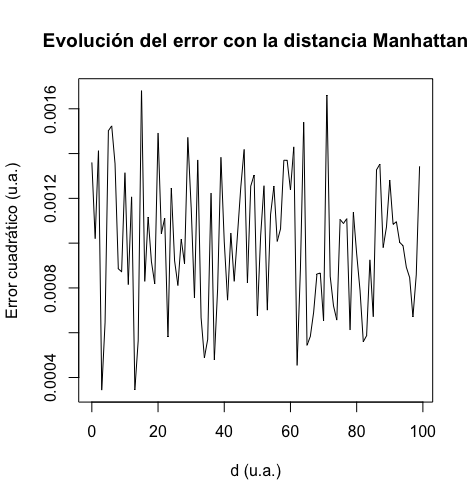
\includegraphics[width=7truecm]{Rplotmanh.png}
%     \caption{Error en función de la distancia en unidades arbitrarias.}
%     \label{fig:my_label}
% \end{figure}

A


%%%%%%%%%%%%%%%%%%%%%%%%%%%%%%%%%%%%%%%%%%%%%%%%%%%%
% Tercera parte: Resultados + Discusión  <--> PEC3 %
%%%%%%%%%%%%%%%%%%%%%%%%%%%%%%%%%%%%%%%%%%%%%%%%%%%%


\chapter{Discusión}

% Discusión de los resultados en el contexto del proyecto. Es en este apartado donde cobran sentido y en el cual se responden las preguntas de investigación y se muestra cómo los resultados dan respuesta a los problemas planteados.

A


%%%%%%%%%%%%%%%%%%%%%%%%%%%%%%%%%%%%%%%%%%%%%%%%%%%%%%%%%%%%%%%%%%%%%%%%%%%%%
% Cuarta parte: Conclusión + Retoques (Glosario, seguimiento...)  <--> PEC4 %
%%%%%%%%%%%%%%%%%%%%%%%%%%%%%%%%%%%%%%%%%%%%%%%%%%%%%%%%%%%%%%%%%%%%%%%%%%%%%


\chapter{Conclusiones y trabajos futuros}

\section{Conclusiones}

% Este capítulo tiene que incluir:
% 
% \begin{itemize}
% \item Una descripción de las conclusiones del trabajo:
% \begin{itemize}
%     \item Una vez se han obtenido los resultados, ¿qué conclusiones se extraen?
%     \item ¿Estos resultados son los esperados? ¿O han sido sorprendentes? ¿Por qué?
% \end{itemize}
% \item Una reflexión crítica sobre el logro de los objetivos planteados inicialmente:
% \begin{itemize}
%     \item ¿Hemos logrado todos los objetivos? Si la respuesta es negativa, ¿por qué motivo?
% \end{itemize}
% \end{itemize}

A


\section{Líneas de futuro}

% Las líneas de trabajo futuro que no se han podido explorar en este trabajo y han quedado pendientes.

A


\section{Seguimiento de la planificación}

% \begin{itemize}
% \item
% Un análisis crítico del seguimiento de la planificación y metodología a lo largo del producto:
% \begin{itemize}
%     \item ¿Se ha seguido la planificación?
%     \item ¿La metodología prevista ha sido suficientemente adecuada?
%     \item ¿Ha habido que introducir cambios para garantizar el éxito del trabajo? ¿Por qué?
% \end{itemize}
% \item De los impactos previstos a \ref{s:etic}, ético-sociales, de sostenibilidad y de diversidad, avaluad/mencionad si se han mitigado (si eran negativos) o si se han conseguido (si eran positivos).
% \item Si han aparecido impactos no previstos en \ref{s:etic}, evaluar/mencionar cómo se han mitigado (si eran negativos) o que han aportado (si eran positivos).
% \end{itemize}

A


% \glossarystyle{list} % Antes de \printglossaries. Estilos (list, altlist, listgroup, listhypergroup)
\printglossaries
% \printglossaries[type=\acronymtype]


\newpage

\listoffigures


\newpage

\listoftables


\newpage

\listofmyequations


\newpage

\bibliography{TFM} 
\bibliographystyle{ieeetr}


%%%%%%%%%%%%%%%%%%%%%%%%
% Secciones opcionales %
%%%%%%%%%%%%%%%%%%%%%%%%


% \newpage
% 
% \appendix
% 
% %Listado de apartados que son demasiado extensos para incluir dentro de la memoria y tienen un carácter autocontenido (por ejemplo, manuales de usuario, manuales de instalación, etc.)
% 
% %Dependiendo del tipo de trabajo, es posible que no haya que añadir algún anexo.
% 
% \chapter{Anexo A}
% 
% \section{Anexo 1}




% -------------------------------------------------------------------------------------------------------%
% -------------------------------------------------------------------------------------------------------%
% ----------------------------------- U  T  I  L  I  D  A  D  E  S --------------------------------------%
% -------------------------------------------------------------------------------------------------------%
% -------------------------------------------------------------------------------------------------------%

% %%%%%%%%%%%%%%%%%%%%%%%%%%%%%%
% % Para introducir ecuaciones %
% %%%%%%%%%%%%%%%%%%%%%%%%%%%%%%
% 
% % Introducir una ecuación numerada y con etiqueta:
% % ------------------------------------------------
% 
% \begin{equation}\label{eq:etiquetaEq}
% Eq
% \end{equation}
% \myequations{Descripción Eq}
% 
% % Referenciar una ecuación:
% % -------------------------
% 
% La ecuación ~\ref{eq:etiquetaEq} es ...
% 
% % Poner paréntesis alrededor de una referencia de ecuación:
% % ---------------------------------------------------------
% 
% La ecuación \eqref{eq:pythagoras} es ...
% 
% % Para introducir ecuaciones no numeradas:
% % ----------------------------------------
% 
% \begin{equation*}
% Eq
% end{equation*}
% \myequations{Descripción Eq}
% 
% % Para introducir ecuaciones con diversas fórmulas:
% % -------------------------------------------------
% 
% \begin{align}
% e^{i\pi} & = \cos(\pi) + i\sin(\pi) \notag \\
%          & = -1 .
% \end{align}
% 
% \begin{equation}
%     1 + 1 = 2
% \end{equation}
% \label{eq:2.1}


% -------------------------------------------------------------------------------------------------------%


\end{document}
